% First reader C; scan 017 only. Unresolved notation is repeated in place.
\scanpage{17}
\mspage{\textcircled{1}}

\diagram{\begin{tikzcd}[ampersand replacement=\&]
\mathbb E_n\arrow[r,shift left,"{\unsure{\delta|\partial}}_n"]\&\mathbb E_{n+1}\arrow[l,shift left,"K_n"]
\end{tikzcd}}
$n\in\mathbb N^*\quad\text{i.e. }n\geq1$

\[
\left.\begin{aligned}
{\unsure{\delta|\partial}}_n &: [1,n]\hookrightarrow[1,n+1]&&\text{inclusion}\\
K_n &: [1,n]\longleftarrow[1,n+1]&&\text{rétraction}
\end{aligned}\right]
\]
\margin{$\unsure{\mathcal G_n|\mathfrak S_n}$ opère sur $\mathbb E_n$
\diagram{\begin{tikzcd}[ampersand replacement=\&]
\unsure{\mathcal G_n|\mathfrak S_n}\arrow[r,hook,"i_n"]\&\unsure{\mathcal G_{n+1}|\mathfrak S_{n+1}}
\end{tikzcd}}}

\margin{${\unsure{\delta|\partial}}_nK_n\overset{\text{déf}}{=}p_{n+1}$ (\unsure{projection|projecteur} dans $\mathbb E_{n+1}$, rétraction sur $\mathbb E_n\subset\mathbb E_{n+1}$}
\figure{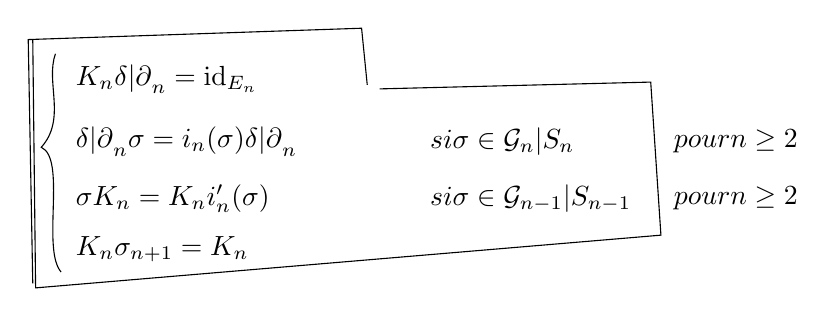
\begin{tikzpicture}[x=.72cm,y=.72cm]
\node[anchor=west,inner sep=0pt] at (0.75,3.2) {$K_n{\unsure{\delta|\partial}}_n=\mathrm{id}_{\mathbb E_n}$};
\node[anchor=west,inner sep=0pt] at (0.75,2.1) {${\unsure{\delta|\partial}}_n\sigma=i_n(\sigma){\unsure{\delta|\partial}}_n$};
\node[anchor=west,inner sep=0pt] at (0.75,1.1) {$\sigma K_n=K_n i^{\prime}_n(\sigma)$};
\node[anchor=west,inner sep=0pt] at (0.75,0.2) {$K_n\sigma_{n+1}=K_n$};
\node[anchor=west,inner sep=0pt] at (7,2.1) {$\text{si }\sigma\in\unsure{\mathcal G_{n}|\mathfrak S_{n}}$};
\node[anchor=west,inner sep=0pt] at (7,1.1) {$\text{si }\sigma\in\unsure{\mathcal G_{n-1}|\mathfrak S_{n-1}}$};
\node[anchor=west,inner sep=0pt] at (11.3,2.1) {$\text{pour }n\geq2$};
\node[anchor=west,inner sep=0pt] at (11.3,1.1) {$\text{pour }n\geq2$};
\draw (.4,3.65)..controls(.22,3.15)and(.6,2.5)..(.15,2.0)..controls(.6,1.8)and(.15,.2)..(.5,-.2);
\draw (0,-.4)--(-.08,3.9)--(5.8,4.1)--(5.9,3.1);
\draw (6.12,3.03)--(10.9,3.15)--(11.08,.45)--(.05,-.48)--(0,3.9);
\end{tikzpicture}}
\margin{où $i'_n\underset{\unsure{\text{déf}}}{=}i_n i_{n-1}:\unsure{\mathcal G_{n-1}|\mathfrak S_{n-1}}\longrightarrow\unsure{\mathcal G_n|\mathfrak S_n}\longrightarrow\unsure{\mathcal G_{n+1}|\mathfrak S_{n+1}}$}
\margin{où $\sigma_m\in\unsure{\mathcal G_m|\mathfrak S_m}$ est la transposition $[m-1,m)$}

\diagram{\begin{tikzcd}[ampersand replacement=\&]
\mathbb E_n^*\arrow[r,shift right=2,"d_n=K_n^*"']\&\mathbb E_{n+1}^*\arrow[l,shift right=2,"p_n={\unsure{\delta|\partial}}_n^*"']
\end{tikzcd}}

\figure{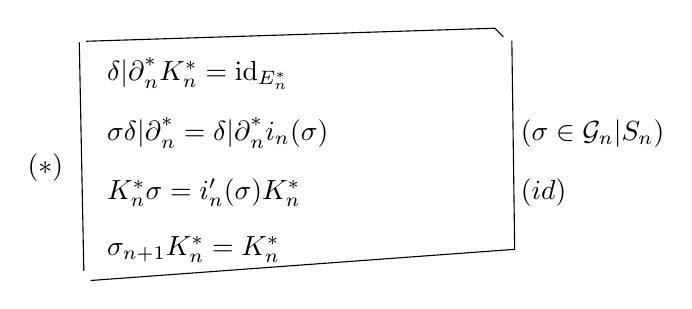
\begin{tikzpicture}[x=.72cm,y=.72cm]
\node[anchor=west,inner sep=0pt] at (-1,1.55) {$(*)$};
\node[anchor=west,inner sep=0pt] at (0.4,3.2) {${\unsure{\delta|\partial}}_n^*K_n^*=\mathrm{id}_{E_n^*}$};
\node[anchor=west,inner sep=0pt] at (0.4,2.15) {$\sigma{\unsure{\delta|\partial}}_n^*={\unsure{\delta|\partial}}_n^*i_n(\sigma)$};
\node[anchor=west,inner sep=0pt] at (0.4,1.1) {$K_n^*\sigma=i^{\prime}_n(\sigma)K_n^*$};
\node[anchor=west,inner sep=0pt] at (0.4,0.1) {$\sigma_{n+1}K_n^*=K_n^*$};
\node[anchor=west,inner sep=0pt] at (7.7,2.15) {$(\sigma\in\unsure{\mathcal G_{n}|\mathfrak S_{n}})$};
\node[anchor=west,inner sep=0pt] at (7.7,1.1) {$\text{(id)}$};
\draw (0,-.28)--(-.08,3.75);
\draw (.04,3.77)--(7.25,4.0)--(7.4,3.85);
\draw (7.55,3.78)--(7.6,.1)--(.12,-.45);
\end{tikzpicture}}
réalisation dans $(\mathrm{Ens})$ de syst. de
$(\text{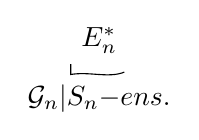
\begin{tikzpicture}[baseline=(e.base)]\node[inner sep=0pt] (e) at (0,0) {$E_n^*$};\draw (-.36,-.3)--(-.36,-.43)..controls(-.12,-.39)and(.12,-.48)..(.32,-.4);\node[anchor=north,inner sep=0pt] at (0,-.55) {$\unsure{\mathcal G_{n}|\mathfrak S_{n}}\text{-ens.}$};\end{tikzpicture}},{\unsure{\delta|\partial}}_n^*,K_n^*)$
satisfaisant aux relations $(*)$, \uline{plus}

\figure{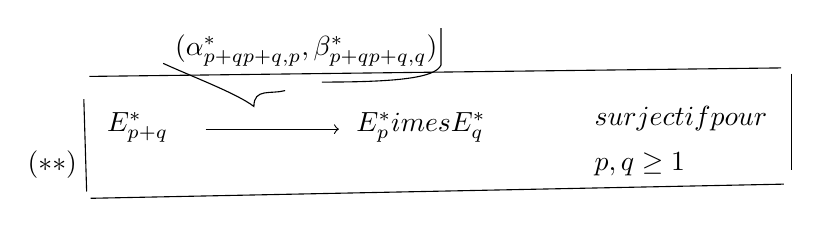
\begin{tikzpicture}[x=.72cm,y=.72cm]
\node[anchor=west,inner sep=0pt] at (-1,0.1) {$(**)$};
\node[anchor=west,inner sep=0pt] at (0.4,0.75) {$E_{p+q}^*$};
\node[anchor=west,inner sep=0pt] at (4.8,0.75) {$E_p^*	imes E_q^*$};
\node[anchor=west,inner sep=0pt] at (9,0.9) {$\text{surjectif pour}$};
\node[anchor=west,inner sep=0pt] at (9,0.1) {$p,q\geq1$};
\node[anchor=west,inner sep=0pt] at (1.6,2.1) {$\inserted{(\alpha^*_{\deleted{\unsure{p+q}}p+q,p},\beta^*_{\deleted{\unsure{p+q}}p+q,q})}$};
\draw[->] (2.15,.72)--(4.5,.72);
\draw (1.4,1.88)..controls(1.9,1.65)and(2.7,1.35)..(3.0,1.12)..controls(3.0,1.45)and(3.3,1.33)..(3.55,1.4);
\draw (4.2,1.55)..controls(5.5,1.55)and(6.2,1.62)..(6.3,1.85)--(6.3,2.5);
\draw (0,1.25)--(.05,-.38);
\draw (.1,1.65)--(12.3,1.8);
\draw (12.48,1.7)--(12.48,.0);
\draw (.12,-.5)--(12.35,-.25);
\end{tikzpicture}}

où
\[
\alpha^*_{n,p}:E_n^*\longrightarrow E_p^*\qquad(n>p\geq1)
\]
défini par
\[
\boxed{\alpha^*_{n,p}={\unsure{\delta|\partial}}_p^*{\unsure{\delta|\partial}}_{p+1}^*\cdots{\unsure{\delta|\partial}}_{n-1}^*}
\]
\diagram{\begin{tikzcd}[ampersand replacement=\&,column sep=small]
E_n^*\arrow[r,"{\unsure{\delta|\partial}}_{n-1}^*"]\&E_{n-1}^*\arrow[r,"{\unsure{\delta|\partial}}_{\unsure{n-2|n-1}}^*"]\&E_{n-2}^*\arrow[r]\&\cdots\arrow[r,"{\unsure{\delta|\partial}}_p^*"]\&E_p^*
\end{tikzcd}}

\[
\beta^*_{n,q}:E_n^*\longrightarrow E_q^*\qquad(n\geq q\geq1)
\]
défini par
\[
\boxed{\beta^*_{n,q}={\unsure{\delta|\partial}}_q^{\prime *}{\unsure{\delta|\partial}}_{q+1}^{\prime *}\cdots{\unsure{\delta|\partial}}_{n-1}^{\prime *}}
\]
\diagram{\begin{tikzcd}[ampersand replacement=\&,column sep=small]
E_n^*\arrow[r,"{\unsure{\delta|\partial}}_{n-1}^{\prime *}"]\&E_{n-1}^*\arrow[r,"{\unsure{\delta|\partial}}_{n-2}^{\prime *}"]\&E_{n-2}^*\arrow[r,phantom,"\cdots"]\&{}\arrow[r,"{\unsure{\delta|\partial}}_q^{\prime *}"]\&E_q^*
\end{tikzcd}}

avec ${\unsure{\delta|\partial}}_m^{\prime *}:E_{m+1}^*\longrightarrow E_m^*$ défini par
\[
\boxed{{\unsure{\delta|\partial}}_m^{\prime *}={\unsure{\delta|\partial}}_m^*\rho_{m+1}^*}
\]
\margin{$\rho_{m+1}^*=\rho_{m+1}^{-1}$ la permutation circu-\newline laire \unsure{élément.} inverse de $\unsure{\mathcal G_{m+1}|\mathfrak S_{m+1}}$}

\margin{$\alpha_{n,p}:\mathbb E_p\hookrightarrow\mathbb E_n$ inclusion canonique
\diagram{\begin{tikzcd}[ampersand replacement=\&,column sep=small]
\beta_{n,q}:\mathbb E_q\arrow[r,hook,no head]\&\mathbb E_n:\quad\beta_{n,q}(i)=i+(n-q)
\end{tikzcd}}
\[
{\unsure{\delta|\partial}}'_{\unsure{m|n}}:\mathbb E_{\deleted{\unsure{m+1}}m}\longrightarrow\mathbb E_{\deleted{\unsure{m}}m+1}
\qquad{\unsure{\delta|\partial}}'_n(i)=i+1
\]}
\[
\text{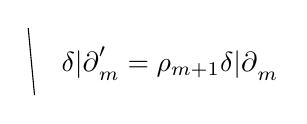
\begin{tikzpicture}[baseline=(e.base)]\node[inner sep=0pt] (e) at (0,0) {${\unsure{\delta|\partial}}'_m=\rho_{m+1}{\unsure{\delta|\partial}}_m$};\draw (-1.8,.45)--(-1.72,-.4);\end{tikzpicture}}
\]
où $\rho_m\in\unsure{\mathcal G_{m+1}|\mathfrak S_{m+1}}$ est la permutation circulaire
\[
\rho_m(i)=\begin{cases}i+1&\text{si }i\in[1,m],\\1&\text{si }i=m+1.\end{cases}
\]
\margin{16}
